\documentclass{article}

\usepackage[a4paper, total={6in, 8in}]{geometry} % Page margins
\usepackage[utf8]{inputenc}
\usepackage{amsmath, amssymb, mathtools, amsfonts, amsthm}
\usepackage{wasysym} % Smiley QED
\usepackage{eulervm} % Font
\usepackage{fancyhdr} % Custom headers and footers
\fancyhead[C]{\thepage} % Page numbering for center header
\usepackage{mdframed}
\usepackage{xcolor}
% list environments               
\usepackage{enumerate}            
\usepackage[shortlabels]{enumitem}      

% Code block environment
\usepackage{listings}            
\lstset{basicstyle = \ttfamily, mathescape}


% figure support
\usepackage{tikz}
\usepackage{graphicx}
\usepackage{subcaption}
\usepackage{import}
\usepackage{xifthen}
\pdfminorversion=7
\usepackage{pdfpages}
\usepackage{transparent}
\newcommand{\incfig}[1]{%
    \def\svgwidth{\columnwidth}
    \import{./figures/}{#1.pdf_tex}
}

\pdfsuppresswarningpagegroup=1

\title{Datastructures \& Algorithms: Exercise 4}
\author{David Sermoneta}


\begin{document}
\maketitle
\section*{Exercise 1.a)}
The array \texttt{C} after line  \texttt{4} looks like the following 
\begin{lstlisting}
    C = [1,3,6].
\end{lstlisting}
After each step of the \texttt{FOR}-loop in line  \texttt{5}, we get the 
following arrays.
\begin{lstlisting}
j = 6) B = [-,-,-,-,-,2]
       C = [1,3,5]
------------------------
j = 5) B = [0,-,-,-,-,2]
       C = [0,3,5]
------------------------
j = 4) B = [0,-,-,-,2,2]
       C = [0,3,4]
------------------------
j = 3) B = [0,-,1,-,2,2]
       C = [0,2,4]
------------------------
j = 2) B = [0,1,1,-,2,2]
       C = [0,1,4]
------------------------
j = 1) B = [0,1,1,2,2,2]
       C = [0,1,3].
\end{lstlisting}

\section*{Exercise 1.b)}
The array  \texttt{A = [2,2,2,2]} gives the desired result. Since then 
at line  \texttt{4}  \texttt{C} will be set to 
\begin{lstlisting}
    C = [0,0,4]
\end{lstlisting}
since the amount of elements smaller than \texttt{0} and  \texttt{1} 
is \texttt{0} for both. 
Each time the \texttt{FOR}-loop runs then, it will decrement \texttt{C[2]}
by $1$. This will happen \texttt{4} times, and so, at the final iteration,
we get that $C = [0,0,0]$.

\section*{Exercise 2a)}
Upon first calling  \texttt{BinarySearch(A, 135, 1, 32)}, a few things
are happening: Firstly, in line \texttt{1.} we check that  
\texttt{1 > 32}, which isn't true, and so go over to line  \texttt{2.}
initialising \texttt{mid =  (first + last)//2 = 16} and now we check
that \texttt{A[16] = 203 == 135} in line \texttt{3.}, which is false, 
and so we go to line  \texttt{4.}, where we check if \texttt{A[mid]} is
larger, which it is, and so we call \texttt{BinarySearch(A, 135, 1, 15)}, 
and repeat the process. Here, again line  \texttt{1.} isn't satisfied,
so we set \texttt{mid = 8}, check that \texttt{A[8] = 119 == 135}, which
isn't true, further it is not larger, so now  we call 
\texttt{BinarySearch(A, 135, 9, 15)}. 
We keep ignoring line \texttt{1.}, we set  \texttt{mid = 12}, check that 
\texttt{A[12] = 175 == 135}, not true, so we check if it is larger, this is
true, so we get to call 
\texttt{BinarySearch(A, 135, 9, 11)}, where we still ignore line 
\texttt{1.}, so we set \texttt{mid = 10}, check if
\texttt{A[10] = 130 == 135}, this doesn't hold, so we check if it is 
bigger -it is not- so we call \texttt{BinarySearch(A, 135, 11, 11)}.
Again, line  \texttt{1.}  is ignored, so we set \texttt{mid = 11}, check
if \texttt{A[11] = 150 == 135}, it isn't, it is however larger, so we call
\texttt{BinarySearch(A, 135, 11, 10)}, where line \texttt{1.} is finally
satisfied, and so we get the return value:
\begin{lstlisting}
    "A does not contain 135"
\end{lstlisting} and we are done.

\section*{Exercise 2.b)}
The optimal choice for jump width  \texttt{m} is $\left\lfloor 
\sqrt{n} \right\rfloor$, that is,  $\left\lfloor 
\sqrt{32} \right\rfloor = $\texttt{m=5}. Since we 
want to find the key \texttt{135}. At  \texttt{i = 1} and 
 \texttt{m = 5} and jump to \texttt{i*m + 1 = 6}, we get that 
 \texttt{L[6] = 108 < 135}, so we increment \texttt{i} by one, and now 
 check \texttt{L[i*m + 1] = L[2*5 + 1] = L[11] = 150}. Since  
 \texttt{150 > 135}, we know that \texttt{135} must be between index 
 \texttt{6} and \texttt{10}, if it's in the list at all.
 So we apply linear search on the sublist \texttt{L[6:10]} and get that
 \texttt{L[7] = 111 < 135}, so we increment by one and get 
 \texttt{L[8] = 119 < 135}, again, increment, and we get the same for 
 all indices until at last \texttt{L[10] = 130 < 135}, which means that
 \texttt{135} is nowhere in the ordered list since it is smaller than
 \texttt{150} and bigger than \texttt{130}, which both are in 
 \texttt{L[10]} and \texttt{L[11]} respectively.

\section*{Exercise 3:}
\begin{lstlisting}[numbers = left]
INORDER-TREE-WALK(x):
    stack = []
    WHILE True:
        IF x != NIL:
            stack.append(x)

            x = x.left

        ELIF: stack != []
            x = stack.pop()
            print(x.key())
            x = x.right
        ELSE:
        break
\end{lstlisting}
The way this algorithm works, is that at first, it will just insert 
elements from top to bottom left into the stack, until we hit the left
most leaf $l_{1}$, which will mean it is the first element we want to print. 
Since the \texttt{WHILE} loop wil run once more when this occur, now 
with \texttt{x = NIL}, and the left most leaf being at the top of the 
stack, this will lead us to set  \texttt{x = $l_1$}, print \texttt{x},
all in accordance to the inorder tree traversal. After that it will set 
 \texttt{x} equal to $l_1$'s right child, and if it exists, everything 
 will go as per usual: We will find the left most leaf of the subtree
 rooted at $l_1$\texttt{.right},  and that will correspond to the second 
 element being printed via the same argument just given. 
\bigskip  \newline
\noindent If $l_1$\texttt{.right = NIL}, then the \texttt{ELIF} statement will 
 just run again making the next \texttt{x} equal to the parent of $l_1$. 
 That element will be printed, following an inorder traversal once again, 
 and then setting the next \texttt{x} equal to its right child, where 
 the argument for getting at the outermost leaf of the tree rooted at 
 that node will be satisfied, exhausting all the cases we can think of. 
 
 \section*{Exercise 4a)}
 I interpret "remove key 2" as meaning to remove the elements 3,6 and 3 
 respectively for each list, and not just the element 2. (The course 
 has been a bit unclear about when what notation means what).
 \begin{figure}[htpb]
     \centering
 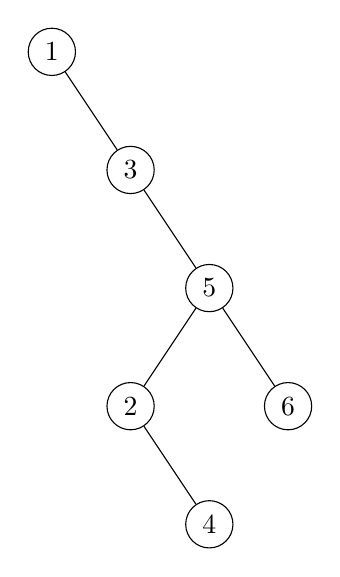
\begin{tikzpicture}[every node/.style={circle, draw, inner sep=2pt, minimum size=6mm}]
     \node (A) at (0,0) {1};
     \node (B) at (1, -1.5) {3};
     \node (C) at (2, -3) {5};
     \node (D) at (1, -4.5) {2};
     \node (E) at (2, -6) {4};
     \node (F) at (3, -4.5) {6};

     \draw (A) -- (B);
     \draw (B) -- (C);
     \draw (C) -- (D);
     \draw (D) -- (E);
     \draw (C) -- (F);
 \end{tikzpicture}
 \caption{Binary search tree built from list a).}
\end{figure}
\begin{figure}[htpb]
     \centering
 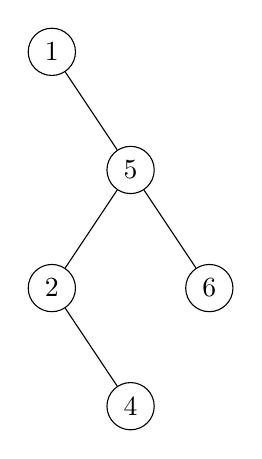
\begin{tikzpicture}[every node/.style={circle, draw, inner sep=2pt, minimum size=6mm}]
     \node (A) at (0,0) {1};
     \node (B) at (1, -1.5) {5};
     \node (C) at (2, -3) {6};
     \node (D) at (0, -3) {2};
     \node (E) at (1, -4.5) {4};

     \draw (A) -- (B);
     \draw (B) -- (C);
     \draw (B) -- (D);
     \draw (D) -- (E);
 \end{tikzpicture}
 \caption{Binary search tree built from list a) after removal of key 2
 (element 3).}
\end{figure}
\newpage

 \section*{Exercise 4b)}
 \begin{figure}[htpb]
    \centering
    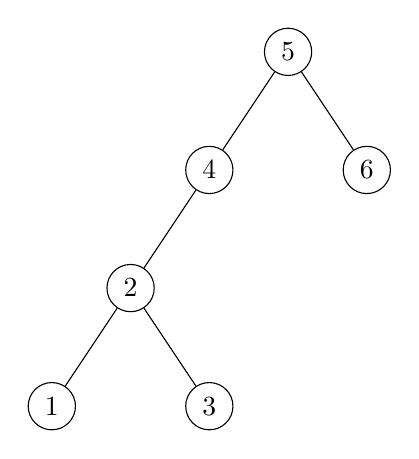
\begin{tikzpicture}[every node/.style={circle, draw, inner sep=2pt, minimum size=6mm}]
     \node (A) at (0,0) {5};
     \node (B) at (1, -1.5) {6};
     \node (C) at (-1, -1.5) {4};
     \node (D) at (-2, -3) {2};
     \node (E) at (-3, -4.5) {1};
     \node (F) at (-1, -4.5) {3};

     \draw (A) -- (B);
     \draw (A) -- (C);
     \draw (C) -- (D);
     \draw (D) -- (E);
     \draw (D) -- (F);
    \end{tikzpicture}
\caption{Binary search tree built from list b).}
\end{figure}
\begin{figure}[htpb]
    \centering
    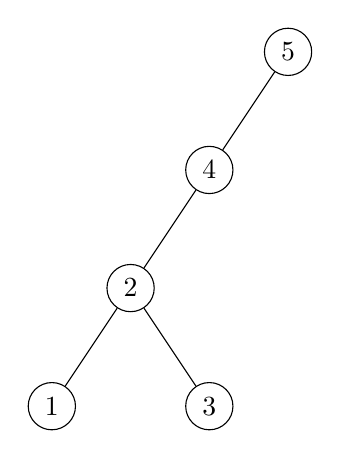
\begin{tikzpicture}[every node/.style={circle, draw, inner sep=2pt, minimum size=6mm}]
     \node (A) at (0,0) {5};
     \node (C) at (-1, -1.5) {4};
     \node (D) at (-2, -3) {2};
     \node (E) at (-3, -4.5) {1};
     \node (F) at (-1, -4.5) {3};

     \draw (A) -- (C);
     \draw (C) -- (D);
     \draw (D) -- (E);
     \draw (D) -- (F);
    \end{tikzpicture}
    \caption{Binary search tree built from list b) after removal of key 2
    (element 6).}
\end{figure}
\newpage

 \section*{Exercise 4c)}
 \begin{figure}[htpb]
     \centering
     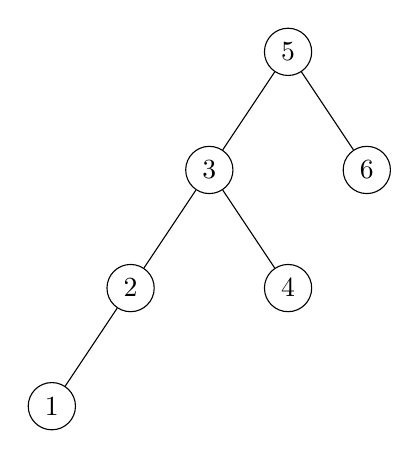
\begin{tikzpicture}[every node/.style={circle, draw, inner sep=2pt, minimum size=6mm}]
     \node (A) at (0,0) {5};
     \node (B) at (1, -1.5) {6};
     \node (C) at (-1, -1.5) {3};
     \node (D) at (-2, -3) {2};
     \node (E) at (0, -3) {4};
     \node (F) at (-3, -4.5) {1};

     \draw (A) -- (B);
     \draw (A) -- (C);
     \draw (C) -- (D);
     \draw (C) -- (E);
     \draw (D) -- (F);
     \end{tikzpicture}
    \caption{Binary search tree built from list c).}
\end{figure}
\begin{figure}[htpb]
     \centering
     \begin{tikzpicture}[every node/.style={circle, draw, inner sep=2pt, minimum size=6mm}]
     \node (A) at (0,0) {5};
     \node (B) at (1, -1.5) {6};
     \node (C) at (-1, -1.5) {4};
     \node (D) at (-2, -3) {2};
     \node (F) at (-3, -4.5) {1};

     \draw (A) -- (B);
     \draw (A) -- (C);
     \draw (C) -- (D);
     \draw (D) -- (F);
     \end{tikzpicture}
    \caption{Binary search tree built from list c) after removal of key 2
    (element 3).}
\end{figure}
\newpage

\section*{Exercise 5:}
\begin{figure}[htpb]
\centering
\begin{tikzpicture}
      \node (A) at (0,0) {50};
      \node (B) at (-3,-1.5) {35};
      \node (C) at (3,-1.5) {60};
      \node (D) at (-4.5,-3) {25};
      \node (E) at (-1.5,-3) {45};
      \node (F) at (1.5,-3) {55};
      \node (G) at (4.5,-3) {65};
      \node (H) at (-5.5,-4.5) {10};
      \node (I) at (-3.5,-4.5) {30};
      \node (J) at (-2.5,-4.5) {40};
      \node (L) at (0.5,-4.5) {51};
      \node (M) at (2.5,-4.5) {56};
      \node (X) at (-4.5,-6) {27};
      \node (Y) at (-3.5,-7.5) {29};
        % Comments
    \node[anchor=west,font=\small] at (A.east) {$^{-2}$};
     \node[anchor=west,font=\small] at (B.east) {$^{-2}$};
     \node[anchor=west,font=\small] at (C.east) {$^{-1}$};
     \node[anchor=west,font=\small] at (D.east) {$^{2}$};
     \node[anchor=west,font=\small] at (E.east) {$^{-1}$};
     \node[anchor=west,font=\small] at (F.east) {$^{0}$};
     \node[anchor=west,font=\small] at (I.east) {$^{-2}$};
     \node[anchor=west,font=\small] at (X.east) {$^{1}$};
      \draw (A) -- (B);
      \draw (A) -- (C);
      \draw (B) -- (D);
      \draw (B) -- (E);
      \draw (C) -- (F);
      \draw (C) -- (G);
      \draw (D) -- (H);
      \draw (D) -- (I);
      \draw (E) -- (J);
      \draw (F) -- (L);
      \draw (F) -- (M);
      \draw (I) -- (X);
      \draw (X) -- (Y);
\end{tikzpicture}
\end{figure}
\newpage
\section*{Exercise 6.a)}
\begin{figure}[htpb]
    \begin{subfigure}[h]{0.4\linewidth}
\begin{tikzpicture}
      \node (A) at (0,0) {10};
      \node (B) at (-1,-1.5) {9};
      \node (C) at (-2,-3) {8};
        % Comments
    \node[anchor=west,font=\small] at (A.east) {$^{-2}$};
     \node[anchor=west,font=\small] at (B.east) {$^{-1}$};
     \node[anchor=west,font=\small] at (C.east) {$^{0}$};
      \draw (A) -- (B);
      \draw (B) -- (C);
\end{tikzpicture}
\caption{Tree before having to do \texttt{RightRot(10)}}
\end{subfigure}
\hfill
\begin{subfigure}[h]{0.4\linewidth}
    \begin{tikzpicture}
      \node (A) at (0,0) {9};
      \node (B) at (1,-1.5) {10};
      \node (C) at (-1,-1.5) {8};
        % Comments
    \node[anchor=west,font=\small] at (A.east) {$^{0}$};
     \node[anchor=west,font=\small] at (B.east) {$^{0}$};
     \node[anchor=west,font=\small] at (C.east) {$^{0}$};
      \draw (A) -- (B);
      \draw (A) -- (C);
    \end{tikzpicture}    
    \caption{Tree after right rotation at vertex \texttt{9}, this is 
    sufficient to lower the $BF(10)$ to 0.}
\end{subfigure}
\hfill
\begin{subfigure}[h]{0.4\linewidth}
    \begin{tikzpicture}
      \node (A) at (0,0) {9};
      \node (B) at (1,-1.5) {10};
      \node (C) at (-1,-1.5) {8};
      \node (D) at (-2, -3) {7};
        % Comments
    \node[anchor=west,font=\small] at (A.east) {$^{-1}$};
     \node[anchor=west,font=\small] at (B.east) {$^{0}$};
     \node[anchor=west,font=\small] at (C.east) {$^{-1}$};
     \node[anchor=west,font=\small] at (D.east) {$^{0}$};
      \draw (A) -- (B);
      \draw (A) -- (C);
      \draw (C) -- (D);
    \end{tikzpicture}    
    \caption{Final Tree!}
\end{subfigure}
\end{figure}
\newpage
\section*{Exercise 6.b)}
\begin{figure}[htpb]
\begin{subfigure}[h]{0.4\linewidth}
    \begin{tikzpicture}
      \node (A) at (0,0) {10};
      \node (B) at (-1,-1.5) {2};
      \node (C) at (1,-1.5) {11};
      \node (D) at (0, -3) {6};
      \node (E) at (2, -3) {17};
      \node (F) at (-1,-4.5) {5};
        % Comments
     \node[anchor=west,font=\small] at (A.east) {$^{-1}$};
     \node[anchor=west,font=\small] at (B.east) {$^{2}$};
     \node[anchor=west,font=\small] at (C.east) {$^{1}$};
     \node[anchor=west,font=\small] at (D.east) {$^{-1}$};
     \node[anchor=west,font=\small] at (E.east) {$^{0}$};
     \node[anchor=west,font=\small] at (F.east) {$^{0}$};
      \draw (A) -- (B);
      \draw (A) -- (C);
      \draw (B) -- (D);
      \draw (D) -- (F);
      \draw (C) -- (E); 
    \end{tikzpicture}    
    \caption{Tree right after adding vertex $5$, giving us an unbalanced 
        tree, with a righ-left case. And so we will need two rotations, 
    one right at $6$ and one left afterwards at $2$.}
\end{subfigure}
\hfill
\begin{subfigure}[h]{0.4\linewidth}
    \begin{tikzpicture}
      \node (A) at (0,0) {10};
      \node (B) at (-1,-1.5) {5};
      \node (C) at (1,-1.5) {11};
      \node (D) at (0, -3) {6};
      \node (E) at (2, -3) {17};
      \node (F) at (-2,-3) {2};
        % Comments
     \node[anchor=west,font=\small] at (A.east) {$^{0}$};
     \node[anchor=west,font=\small] at (B.east) {$^{0}$};
     \node[anchor=west,font=\small] at (C.east) {$^{1}$};
     \node[anchor=west,font=\small] at (D.east) {$^{0}$};
     \node[anchor=west,font=\small] at (E.east) {$^{0}$};
     \node[anchor=west,font=\small] at (F.east) {$^{0}$};
      \draw (A) -- (B);
      \draw (A) -- (C);
      \draw (B) -- (D);
      \draw (B) -- (F);
      \draw (C) -- (E); 
    \end{tikzpicture}    
    \caption{This is the tree after the necessary right and left 
    rotations at the previously specified vertices.}
\end{subfigure}
\hfill
\begin{subfigure}[h]{0.4\linewidth}
    \begin{tikzpicture}
      \node (A) at (0,0) {10};
      \node (B) at (-1,-1.5) {5};
      \node (C) at (1,-1.5) {11};
      \node (D) at (0, -3) {6};
      \node (E) at (2, -3) {17};
      \node (F) at (-2,-3) {2};
      \node (G) at (-1,-4.5) {4};
        % Comments
     \node[anchor=west,font=\small] at (A.east) {$^{-1}$};
     \node[anchor=west,font=\small] at (B.east) {$^{-1}$};
     \node[anchor=west,font=\small] at (C.east) {$^{1}$};
     \node[anchor=west,font=\small] at (D.east) {$^{0}$};
     \node[anchor=west,font=\small] at (E.east) {$^{0}$};
     \node[anchor=west,font=\small] at (F.east) {$^{1}$};
     \node[anchor=west,font=\small] at (G.east) {$^{0}$};
      \draw (A) -- (B);
      \draw (A) -- (C);
      \draw (B) -- (D);
      \draw (B) -- (F);
      \draw (F) -- (G);
      \draw (C) -- (E); 
    \end{tikzpicture}    
    \caption{Final tree!}
\end{subfigure}
\end{figure}

\newpage
\section*{Exercise 7:}
Removing the key \texttt{15} from $T$ involves first searching for the
smallest key in the right subtree rooted at  \texttt{15.right},
replace  \texttt{15} with that key, and then delete \texttt{15} at the new
position. This only involves looking for the leaf \texttt{16}, as that 
satisfies the conditions, setting it as the new root of the tree, and this
gives us the following tree.
\begin{figure}[htpb]
\begin{subfigure}[h]{0.4\linewidth}
    \begin{tikzpicture}
      \node (A) at (0,0) {16};
      \node (B) at (-1,-1.5) {7};
      \node (C) at (1,-1.5) {23};
      \node (E) at (2, -3) {25};
      \node (F) at (-2,-3) {6};
      \node (G) at (1,-4.5) {24};
        % Comments
     \node[anchor=west,font=\small] at (A.east) {$^{1}$};
     \node[anchor=west,font=\small] at (B.east) {$^{-1}$};
     \node[anchor=west,font=\small] at (C.east) {$^{2}$};
     \node[anchor=west,font=\small] at (E.east) {$^{-1}$};
     \node[anchor=west,font=\small] at (F.east) {$^{0}$};
     \node[anchor=west,font=\small] at (G.east) {$^{0}$};
      \draw (A) -- (B);
      \draw (A) -- (C);
      \draw (B) -- (F);
      \draw (E) -- (G);
      \draw (C) -- (E); 
    \end{tikzpicture}    
    \caption{Tree after deleting key \texttt{15}. Now we need to
    balance the subtree rooted at \texttt{23}, which we do by applying 
a double rotation, first a right one at \texttt{25}, and then a left one 
at \texttt{23}. }
\end{subfigure}
\hfill
\begin{subfigure}[h]{0.4\linewidth}
    \begin{tikzpicture}
      \node (A) at (0,0) {16};
      \node (B) at (-1,-1.5) {7};
      \node (C) at (1,-1.5) {23};
      \node (E) at (2, -3) {24};
      \node (F) at (-2,-3) {6};
      \node (G) at (3,-4.5) {25};
        % Comments
     \node[anchor=west,font=\small] at (A.east) {$^{1}$};
     \node[anchor=west,font=\small] at (B.east) {$^{-1}$};
     \node[anchor=west,font=\small] at (C.east) {$^{2}$};
     \node[anchor=west,font=\small] at (E.east) {$^{1}$};
     \node[anchor=west,font=\small] at (F.east) {$^{0}$};
     \node[anchor=west,font=\small] at (G.east) {$^{0}$};
      \draw (A) -- (B);
      \draw (A) -- (C);
      \draw (B) -- (F);
      \draw (E) -- (G);
      \draw (C) -- (E); 
    \end{tikzpicture}    
    \caption{Tree after right rotation at \texttt{25}.}
\end{subfigure}
\hfill
\begin{subfigure}[h]{0.4\linewidth}
    \begin{tikzpicture}
      \node (A) at (0,0) {16};
      \node (B) at (-1,-1.5) {7};
      \node (C) at (1,-1.5) {24};
      \node (E) at (2, -3) {25};
      \node (F) at (-2,-3) {6};
      \node (G) at (0,-3) {23};
        % Comments
     \node[anchor=west,font=\small] at (A.east) {$^{0}$};
     \node[anchor=west,font=\small] at (B.east) {$^{-1}$};
     \node[anchor=west,font=\small] at (C.east) {$^{0}$};
     \node[anchor=west,font=\small] at (E.east) {$^{0}$};
     \node[anchor=west,font=\small] at (F.east) {$^{0}$};
     \node[anchor=west,font=\small] at (G.east) {$^{0}$};
      \draw (A) -- (B);
      \draw (A) -- (C);
      \draw (B) -- (F);
      \draw (C) -- (G);
      \draw (C) -- (E); 
    \end{tikzpicture}    
    \caption{Tree after left rotation at \texttt{23}.}
\end{subfigure}
\end{figure}
\newpage
\section*{Exercise 8:}
\begin{figure}[htpb]
\begin{subfigure}[h]{0.4\linewidth}
    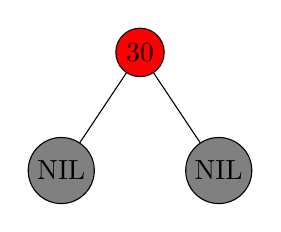
\begin{tikzpicture}[every node/.style={circle, draw, inner sep=2pt, 
        minimum size=6mm}]
        \node[fill= red] (A) at (0,0) {30};
        \node[fill = gray] (B) at (-1, -1.5) {NIL};
        \node[fill = gray] (C) at (1, -1.5) {NIL};

        \draw (A) -- (B);
        \draw (A) -- (C);
    \end{tikzpicture} 
    \caption{Tree after insertion of \texttt{30}.}
\end{subfigure}
\hfill
\begin{subfigure}[h]{0.4\linewidth}
    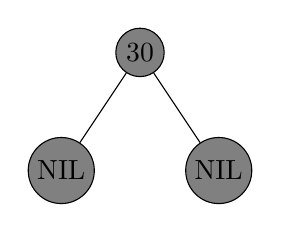
\begin{tikzpicture}[every node/.style={circle, draw, inner sep=2pt, 
        minimum size=6mm}]
        \node[fill= gray] (A) at (0,0) {30};
        \node[fill = gray] (B) at (-1, -1.5) {NIL};
        \node[fill = gray] (C) at (1, -1.5) {NIL};

        \draw (A) -- (B);
        \draw (A) -- (C);
    \end{tikzpicture}
\caption{after recoloring to preserve RB property 1.b}
\end{subfigure}
\hfill
\begin{subfigure}[h]{0.4\linewidth}
    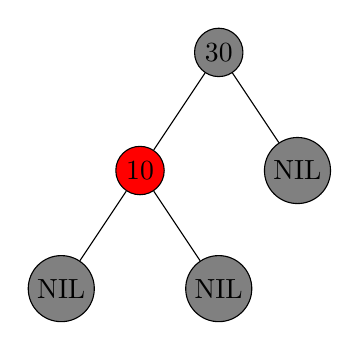
\begin{tikzpicture}[every node/.style={circle, draw, inner sep=2pt, 
        minimum size=6mm}]
        \node[fill= gray] (A) at (0,0) {30};
        \node[fill = red] (B) at (-1, -1.5) {10};
        \node[fill = gray] (C) at (1, -1.5) {NIL};
        \node[fill = gray] (D) at (-2, -3) {NIL};
        \node[fill = gray] (E) at (0, -3) {NIL};

        \draw (A) -- (B);
        \draw (A) -- (C);
        \draw (B) -- (D);
        \draw (B) -- (E);
    \end{tikzpicture} 
\caption{RB property satisfied when inserting \texttt{10}}
\end{subfigure}
\end{figure}
\begin{figure}[htpb]
\begin{subfigure}[h]{0.4\linewidth}
    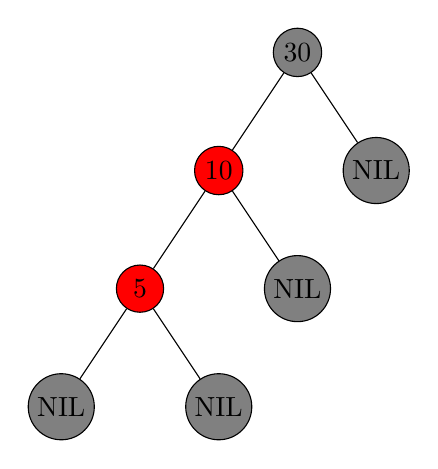
\begin{tikzpicture}[every node/.style={circle, draw, inner sep=2pt, 
        minimum size=6mm}]
        \node[fill= gray] (A) at (0,0) {30};
        \node[fill = red] (B) at (-1, -1.5) {10};
        \node[fill = gray] (C) at (1, -1.5) {NIL};
        \node[fill = red] (D) at (-2, -3) {5};
        \node[fill = gray] (E) at (0, -3) {NIL};
        \node[fill = gray] (F) at (-3, -4.5) {NIL};
        \node[fill = gray] (G) at (-1, -4.5) {NIL};

        \draw (A) -- (B);
        \draw (A) -- (C);
        \draw (B) -- (D);
        \draw (B) -- (E);
        \draw (D) -- (F);
        \draw (D) -- (G);
    \end{tikzpicture} 
\caption{After insertion of \texttt{5}.}
\end{subfigure}

\begin{subfigure}[h]{0.4\linewidth}
    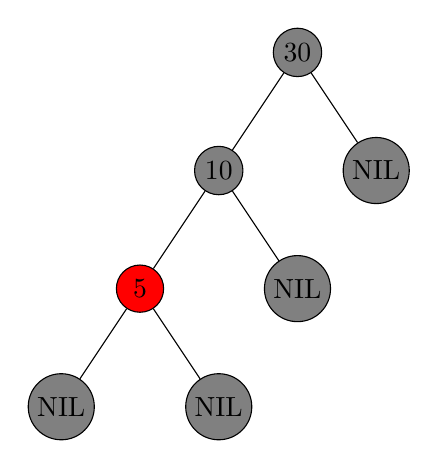
\begin{tikzpicture}[every node/.style={circle, draw, inner sep=2pt, 
        minimum size=6mm}]
        \node[fill= gray] (A) at (0,0) {30};
        \node[fill = gray] (B) at (-1, -1.5) {10};
        \node[fill = gray] (C) at (1, -1.5) {NIL};
        \node[fill = red] (D) at (-2, -3) {5};
        \node[fill = gray] (E) at (0, -3) {NIL};
        \node[fill = gray] (F) at (-3, -4.5) {NIL};
        \node[fill = gray] (G) at (-1, -4.5) {NIL};

        \draw (A) -- (B);
        \draw (A) -- (C);
        \draw (B) -- (D);
        \draw (B) -- (E);
        \draw (D) -- (F);
        \draw (D) -- (G);
    \end{tikzpicture} 
\caption{Recoloring according to line 12, we now have that RB property is
not satisfied, as all paths from any node do not contain equal black nodes.}
\end{subfigure}
\end{figure}
\begin{figure}[htpb]
\begin{subfigure}[h]{0.4\linewidth}
    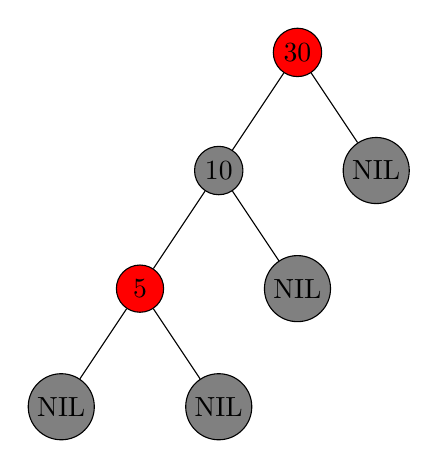
\begin{tikzpicture}[every node/.style={circle, draw, inner sep=2pt, 
        minimum size=6mm}]
        \node[fill= red] (A) at (0,0) {30};
        \node[fill = gray] (B) at (-1, -1.5) {10};
        \node[fill = gray] (C) at (1, -1.5) {NIL};
        \node[fill = red] (D) at (-2, -3) {5};
        \node[fill = gray] (E) at (0, -3) {NIL};
        \node[fill = gray] (F) at (-3, -4.5) {NIL};
        \node[fill = gray] (G) at (-1, -4.5) {NIL};

        \draw (A) -- (B);
        \draw (A) -- (C);
        \draw (B) -- (D);
        \draw (B) -- (E);
        \draw (D) -- (F);
        \draw (D) -- (G);
    \end{tikzpicture} 
\caption{We have changed color of \texttt{30} via line 13.}
\end{subfigure}
\hfill
\begin{subfigure}[h]{0.4\linewidth}
    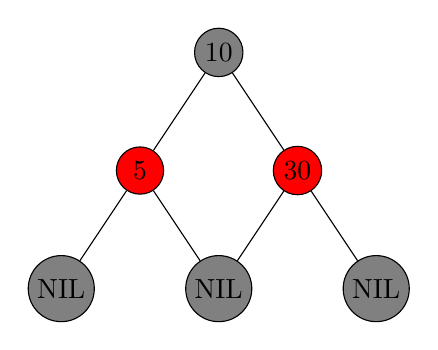
\begin{tikzpicture}[every node/.style={circle, draw, inner sep=2pt, 
        minimum size=6mm}]
        \node[fill= gray] (A) at (0,0) {10};
        \node[fill = red] (B) at (-1, -1.5) {5};
        \node[fill = red] (C) at (1, -1.5) {30};
        \node[fill = gray] (D) at (-2, -3) {NIL};
        \node[fill = gray] (E) at (0, -3) {NIL};
        \node[fill = gray] (F) at (2, -3) {NIL};


        \draw (A) -- (B);
        \draw (A) -- (C);
        \draw (B) -- (D);
        \draw (B) -- (E);
        \draw (C) -- (F);
        \draw (C) -- (E);
    \end{tikzpicture} 
\caption{We have done a right rotation on \texttt{30}, getting our final
tree, satisfying the RB property!}
\end{subfigure}
\end{figure}
\newpage
\section*{Exercise 9:}
\begin{center}

\[
\begin{tabular}{cccccccc}
 index & 0 & 1 & 2 & 3 & 4 & 5 & 6 \\[0pt]
\hline key &  &  & $\mathbf{9}$ &  &  &  &  \\[0pt]
 i &  &  & 0 &  &  &  &  \\[0pt]
\end{tabular}
\]

\[
\begin{tabular}{cccccccc}
 index & 0 & 1 & 2 & 3 & 4 & 5 & 6 \\[0pt]
\hline key &  &  & 9 &  &  & $\mathbf{12}$ &  \\[0pt]
 i &  &  & 0 &  &  & 0 &  \\[0pt]
\end{tabular}
\]

\[
\begin{tabular}{cccccccc}
 index & 0 & 1 & 2 & 3 & 4 & 5 & 6 \\[0pt]
\hline key & $\mathbf{5}$ &  & 9 &  &  & 12 &  \\[0pt]
 i & 1 &  & 0 &  &  & 0 &  \\[0pt]
\end{tabular}
\]

\[
\begin{tabular}{cccccccc}
 index & 0 & 1 & 2 & 3 & 4 & 5 & 6 \\[0pt]
\hline key & 5 &  & 9 & $\mathbf{3}$ &  & 12 &  \\[0pt]
 i & 1 &  & 0 & 0 &  & 0 &  \\[0pt]
\end{tabular}
\]

\[
\begin{tabular}{cccccccc}
 index & 0 & 1 & 2 & 3 & 4 & 5 & 6 \\[0pt]
\hline key & 5 &  & 9 & 3 & $\mathbf{7}$ & 12 &  \\[0pt]
 i & 1 &  & 0 & 0 & 2 & 0 &  \\[0pt]
\end{tabular}
\]
\end{center}


\section*{Exercise 10:}
\begin{proof}
A little bird whispers in my ear and tells me to read the first code as 
hexadecimal ascii representations of characters. That is, the integer 
\texttt{54} should be interpreted as the character $\mathbf{T}$, as
that is the hexadecimal ascii representation of the character  
$\mathbf{T}$. Following the bird's advice, we get the string 
\begin{center}
    \texttt{T h e SP a n s w e r SP is : SP 4 2},
\end{center} which in natural language becomes 
\begin{center}
    The answer is: 42.
\end{center}
Just like in exercise 1, we want to translate the number 
$240743138$ to its representation in base 128, where then each coefficient
will translate to an ascii character in decimal form. That is, we want
to find the coefficients $a_{k}$ to the equation 
\[
240743138 = \sum\limits_{k=0}^{N} a_{k}\cdot 128^k.
\] 
By using the euclidean algorithm, we get that each iteration 
$r_{i}$ will give us the coefficient $a_{i}$. For example, since 
\[  240743138 = 98,\]
we know that $a_0 = 98$. Then we can take the difference of these two, 
and divide it by  $128$, to get the integer \[
    \frac{1240743138 - 98}{128} =880805.
\] Repeating this process until it terminates (that the euclidean 
algorithm terminates is omitted in this assignent) yields the coefficients 
\begin{align*}
    a_0 =&  98 \\
    a_1 =& 101 \\
    a_2 =& 101 \\
    a_3 =& 114, 
\end{align*} after which the program terminates. Translating these into
their decimal ascii counterparts gives us the characters 
\begin{alignat*}{4}
    & a_0 \quad && a_1  \quad && a_2 \quad  && a_3 \\
    & 98   && 101 && 101 &&  114 \\
    & b && e && e && r
\end{alignat*}
And so the holy recipe of liquid bread is $\mathbf{beer}$.
\end{proof}
\end{document}

